\clearpage
\subsection{Statement} % (fold)
\label{sub:statement}

When you are created a program you define the actions the computer will perform when the program is run. Each of these \emph{actions} is coded as a \textbf{statement} within the program. This style of programming is known as \textbf{imperative} programming. Imperative means to give authoritative commands, and that is what we do in our programs. Our programs are lists of \emph{authoritative commands}, statements, that \emph{tell} the computer the actions it is to perform.

\begin{figure}[h]
   \centering
   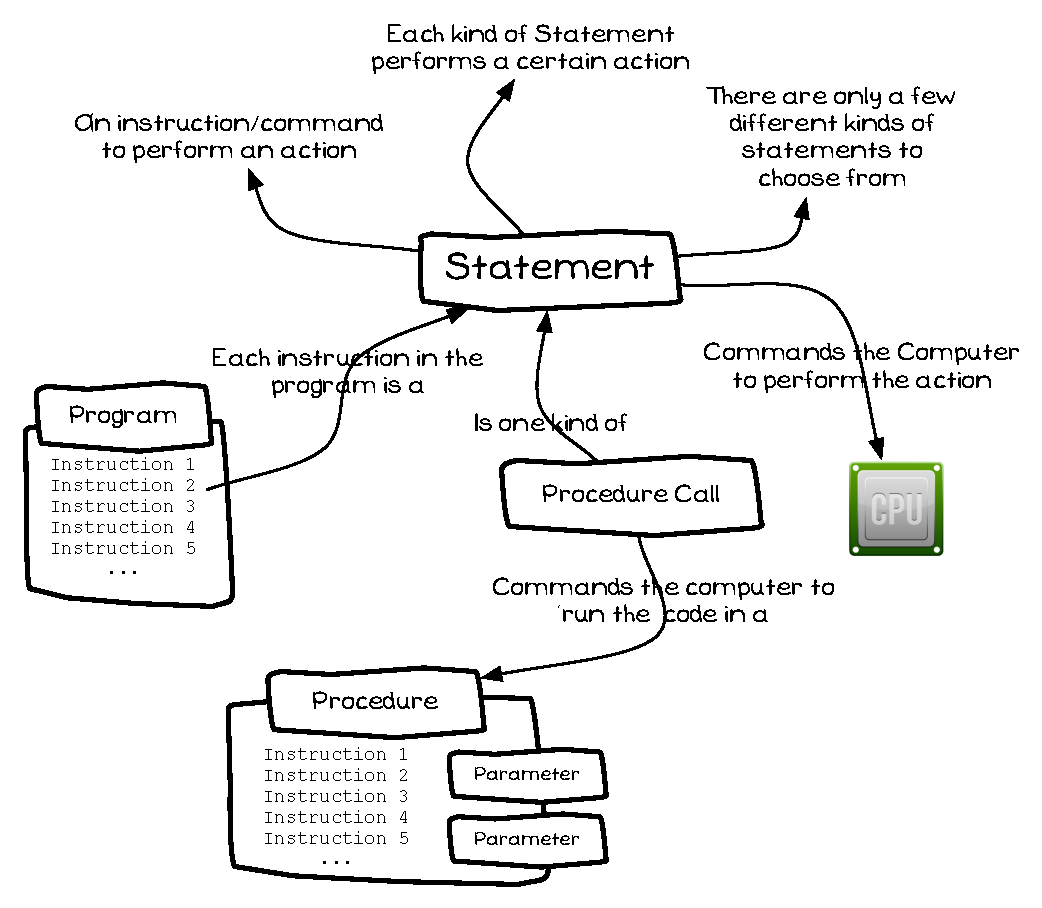
\includegraphics[width=\textwidth]{./topics/program-creation/diagrams/Statement} 
   \caption{A statement is a command for the computer to perform an action}
   \label{fig:program-creation-statement}
\end{figure}


\mynote{
\begin{itemize}
  \item A statement is a \textbf{term} used to describe the instructions in your code.
  \item Figure \ref{fig:program-creation-statement} shows the concepts related to statements.
  \item A statement is a \textbf{command}, an instruction to perform an action.
  \item A \nameref{sub:program} has a list of statements that are followed when it is executed.
  \item There are only a few kinds of statements. Each statement has a defined set of actions the computer performs to carry out the \emph{command}.
  \item A \nameref{sub:procedure call} is a kind of statement that tells the computer to run the code in a \nameref{sub:procedure}.
\end{itemize}
}

% section statement (end)